%%% Fun stuff:
%\footnote{NGC 2146 - ESA/Hubble \& NASA}
%
%\begin{itemize}
%\item Item 1 
%\item Item 2
%\end{itemize}
%
%\begin{figure}
%\fbox{\includegraphics[width=8cm]{figure.jpg}}
%\end{figure}
%
%\center{\alert{Bright Red Text}}
%
%\begin{block}{Text above the block}
%\begin{figure}
%\includegraphics[width=9cm]{figure.jpb}
%\end{figure}
%\end{block}
%
%\uncover<2>{This text will show up on the second slide.}
%
%\invisible<2>{This text will be invisible on the second slide.}
%
%\begin{columns}[c]
%\column{.6 \textwidth}
%First column text
%\begin{itemize}
%\item Item 1
%\end{itemize}
%\column{.2 \textwidth}
%Second column text
%\end{columns}

\documentclass[blue,serif]{beamer}


\usepackage{datetime}
\usepackage[dark]{beamerthemesidebar}
\usepackage[english]{babel}
\usepackage{graphicx}
\usepackage{amsmath}
\usepackage{amssymb}
%\usepackage[dvipsnames]{xcolor}
\usepackage{xcolor}
%\usepackage[latin1]{inputenc}
%\renewcommand{\thefootnote}{}
%\usepackage{times}
%\usepackage[T1]{fontenc}
%\beamertemplatenavigationsymbolsempty

\setbeamertemplate{enumerate item}{(\alph{enumi})}
\setbeamertemplate{enumerate subitem}{(\roman{enumii})}

\def\be{\begin{equation*}}
\def\ee{\end{equation*}}
\def\bea{\begin{eqnarray*}}
\def\eea{\end{eqnarray*}}

\title[Side Deck - Capsone 2]
      {Side Deck - Capstone 2}

\subject{Side Deck - Capstone 2}

\begin{document}

\addtobeamertemplate{footline}{
  \setlength\unitlength{1ex}
  \begin{picture}(0,0) 
    % \put{} defines the position of the frame
    \put(0,0){\makebox(0,0)[bl]{
    
\includegraphics[width=2.5cm]{figures/springboard logo-1.png}
   % \includegraphics{figures/image2.png}
 %   \includegraphics{figures/image3.png}
    }}
  \end{picture}%
}{}

%%%%%%%%%%%%%%%%%%%%%%%%%%%%%%
%%%%% Slides Start Here %%%%%%
%%%%%%%%%%%%%%%%%%%%%%%%%%%%%%

\begin{frame}{Leveraging customer information for strategic telemarketing in the banking industry }

\usebackgroundtemplate{
\includegraphics[width=\paperwidth]{figures/fig_bank_image.jpg}}

\begin{columns}[c]
\column{.6 \textwidth}
  \begin{figure}

\includegraphics[width=5cm]{figures/logo_telemarketing.jpg}
 \end{figure}
  \vspace{-.4cm}
\column{.4\textwidth}
%  \textBig{Capstone 2 project presentation}
   \center{\textbf{Author:} Isaac Ghebregziabher} \vspace{-.1cm}
%   \center{\textbf{Supervisor:} Yuxian Xin}
%   \vspace{-.3cm}
    \center{Capstone Project two}
    \center{\today}
\end{columns}
%\center{Capstone Project One}
%\vspace{0.2cm}
%\vspace{-.3cm}


\end{frame}

%%%%%%%%%%%%%%%%%%%%%%%%%%%%%%
%%%%%%%%%%%%%%%%%%%%%%%%%%%%%%
\section{Introduction} %%%%
%%%%%%%%%%%%%%%%%%%%%%%%%%%%%%
%%%%%%%%%%%%%%%%%%%%%%%%%%%%%%

\begin{frame}{What is telemarketing?}
%\linespread{1.3}

%\begin{columns}
%	\column{.6 \textwidth}
\begin{quote}
Telemarketing is a method of direct marketing in which a salesperson solicits prospective customers to buy products or services, either over the phone or through a subsequent face to face or web conferencing appointment scheduled during the call.
\end{quote}

\end{frame}


\begin{frame}{Telemarketing cost has been increasing in the banking industry}
%\linespread{1.3}

%\begin{columns}
%	\column{.6 \textwidth}
\begin{itemize}
   \item Bank marketing cost increased over two years
	\item Cost as high as 0.15\% of total bank's asset 
%	\item Fast and reliable diagnostic is needed
\end{itemize}

%	\column{.4 \textwidth}
	\begin{figure}
		
		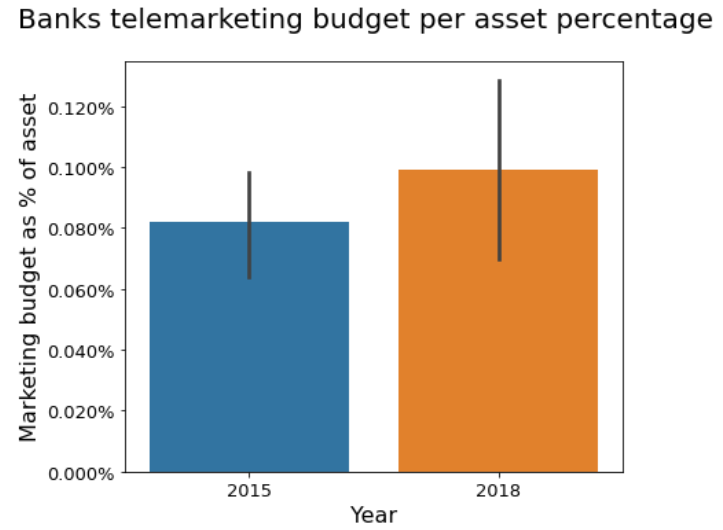
\includegraphics[width=6.0cm]{figures/fig_bank_marketing_budget.PNG}
%		\caption{Single valued features (dropped).}
	\end{figure}
%\end{columns}
Predictive modeling could increase marketing success

\end{frame}


%%%%%%%%%%%%%%%%%%%%%%%%%%%%%%
%%%%%%%%%%%%%%%%%%%%%%%%%%%%%%
\subsection{Objective} %%%%
%%%%%%%%%%%%%%%%%%%%%%%%%%%%%%
%%%%%%%%%%%%%%%%%%%%%%%%%%%%%%

\begin{frame}{Object and project deliverable}
%\linespread{1.3}

%\begin{columns}
%	\column{.6 \textwidth}
\textbf{Deliverable:} ML model for predicting whether a customer will subscribe to a term-deposit
 \begin{quote} A term deposit is a fixed-term investment that includes the deposit of money into an account at a financial institution
 \end{quote}
\begin{itemize}
	\item The developed model will help the bank:
	\begin{itemize}
	    \item Cluster its customers into meaningful groups
	    \item Predict customer response to its telemarketing campaigns
	    \item Identify target customer groups for its future tele-marketing campaigns
	\end{itemize}
	
%	\item Raman Scattered light is signature of molecular composition
%	\item Fast and reliable diagnostic is needed
\end{itemize}

%	\column{.4 \textwidth}
%	\begin{figure}
		
%		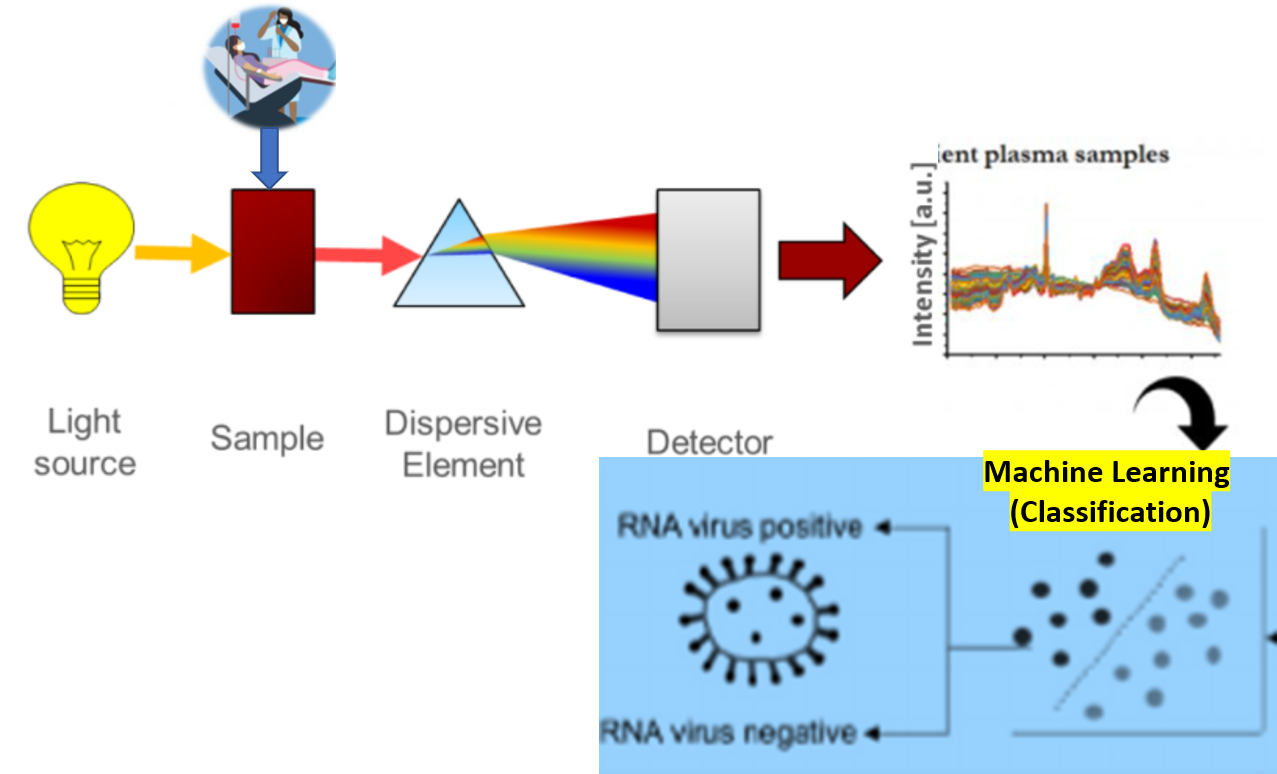
\includegraphics[width=9.0cm]{figures/covid_raman_and_ML.png}
%		\caption{Single valued features (dropped).}
%	\end{figure}
%\end{columns}


\end{frame}

\subsection{Stakeholders}
\begin{frame}{Stakeholders and telemarketing data}
%\linespread{1.3}
-- Our client is a Portuguese banking institution.\\
-- Brought to us data related to telemarketing campaign\\
-- The data consists of the following details:\\
\linespread{1.3}
%\begin{columns}
%	\column{.6 \textwidth}
\begin{itemize}
    \item \textbf{Demographics} (age, job, education, marital status),
    \item \textbf{Financial data} (credit, housing loan, personal loan),
	\item \textbf{Contact details} (such as method of contact and month)
	\item \textbf{Previous campaign data} (such as outcome of previous campaign)
%	\item Last column `\textit{\textbf{diagnostic}}' is target #variable
\end{itemize}
\end{frame}


%%%%%%%%%%%%%%%%%%%%%%%%%%%%%%
%%%%%%%%%%%%%%%%%%%%%%%%%%%%%%
\section{Data Wrangling} %%%%
%%%%%%%%%%%%%%%%%%%%%%%%%%%%%%
%%%%%%%%%%%%%%%%%%%%%%%%%%%%%%

\begin{frame}{Overview of the Dataset}
%\linespread{1.3}

%\begin{columns}
%	\column{.6 \textwidth}
\begin{itemize}
    \item 45211 rows X 17 columns
    \item 7 integer and 10 categorical type features
	\item No duplicates and missing values
%	\item Last column `\textit{\textbf{diagnostic}}' is target #variable
\end{itemize}

%	\column{.4 \textwidth}
	\begin{figure}
		
		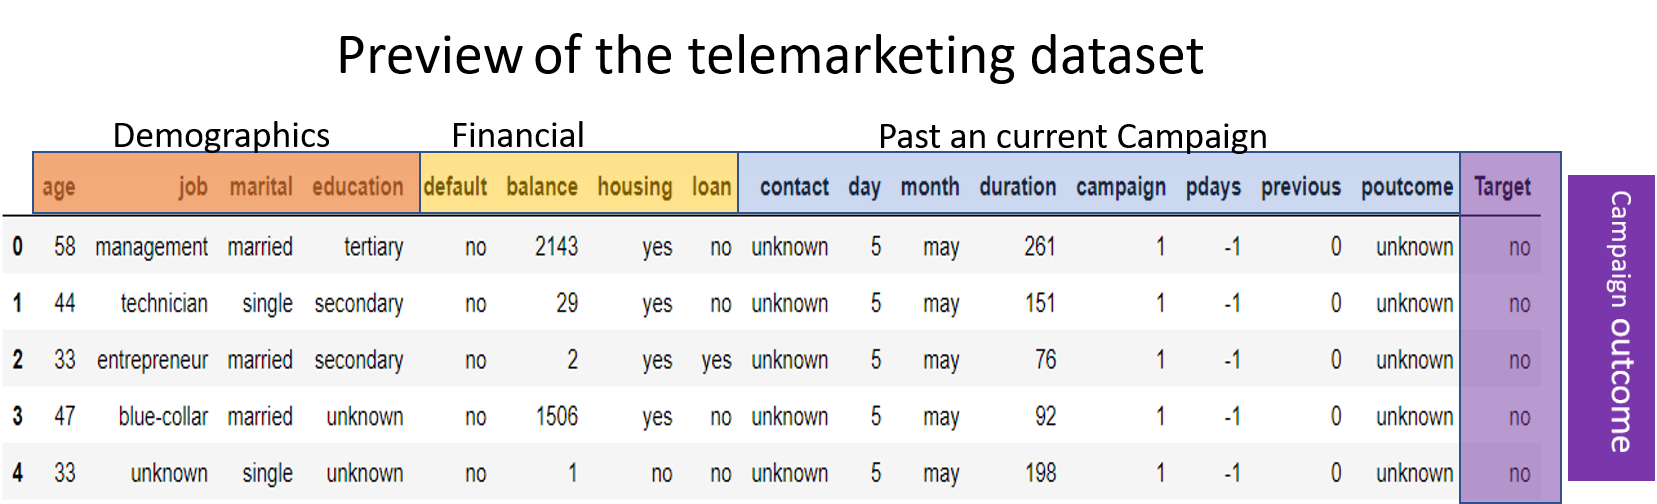
\includegraphics[width=9.0cm]{figures/fig_bank_dataset.png}
%		\caption{Single valued features (dropped).}
	\end{figure}
%\end{columns}


\end{frame}

\begin{frame}{Categorical feature exploration – Demographic segmentation}
%\linespread{1.3}

%\begin{columns}
%	\column{.6 \textwidth}
\begin{itemize}
    \item 12 job categories
	\item 3 marital status groups
	\item 4 educational levels including 1 unknown
\end{itemize}

%	\column{.4 \textwidth}
	\begin{figure}
		
		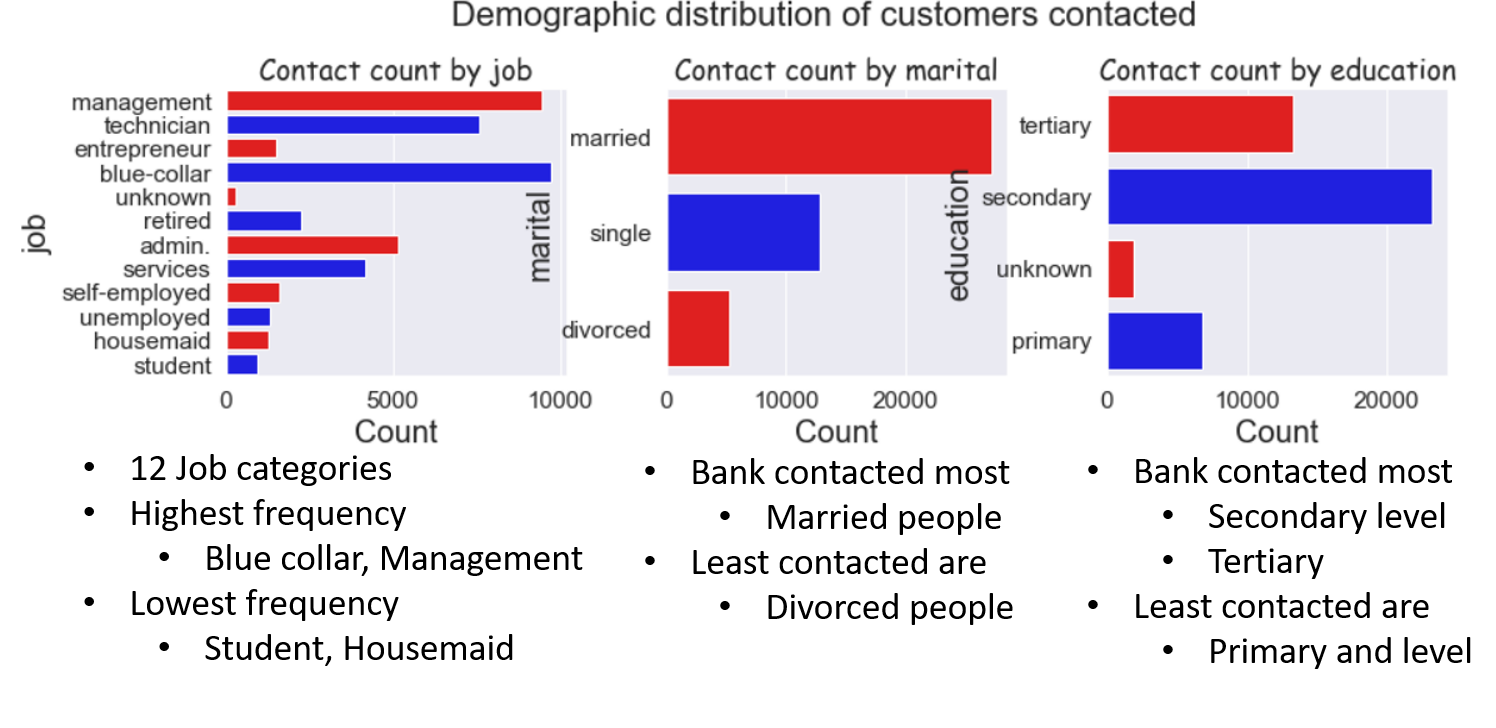
\includegraphics[width=9.0cm]{figures/fig_cat_demo_count.png}
%		\caption{Single valued features (dropped).}
	\end{figure}
%\end{columns}


\end{frame}

\begin{frame}{Categorical feature exploration – past and current campaign details}
%\linespread{1.3}

%\begin{columns}
%	\column{.6 \textwidth}
%\begin{itemize}
%    \item default - Has credit?
%	\item housing - Has housing loan?
%	\item loan - has personal loan?
%\end{itemize}

%	\column{.4 \textwidth}
	\begin{figure}
		
		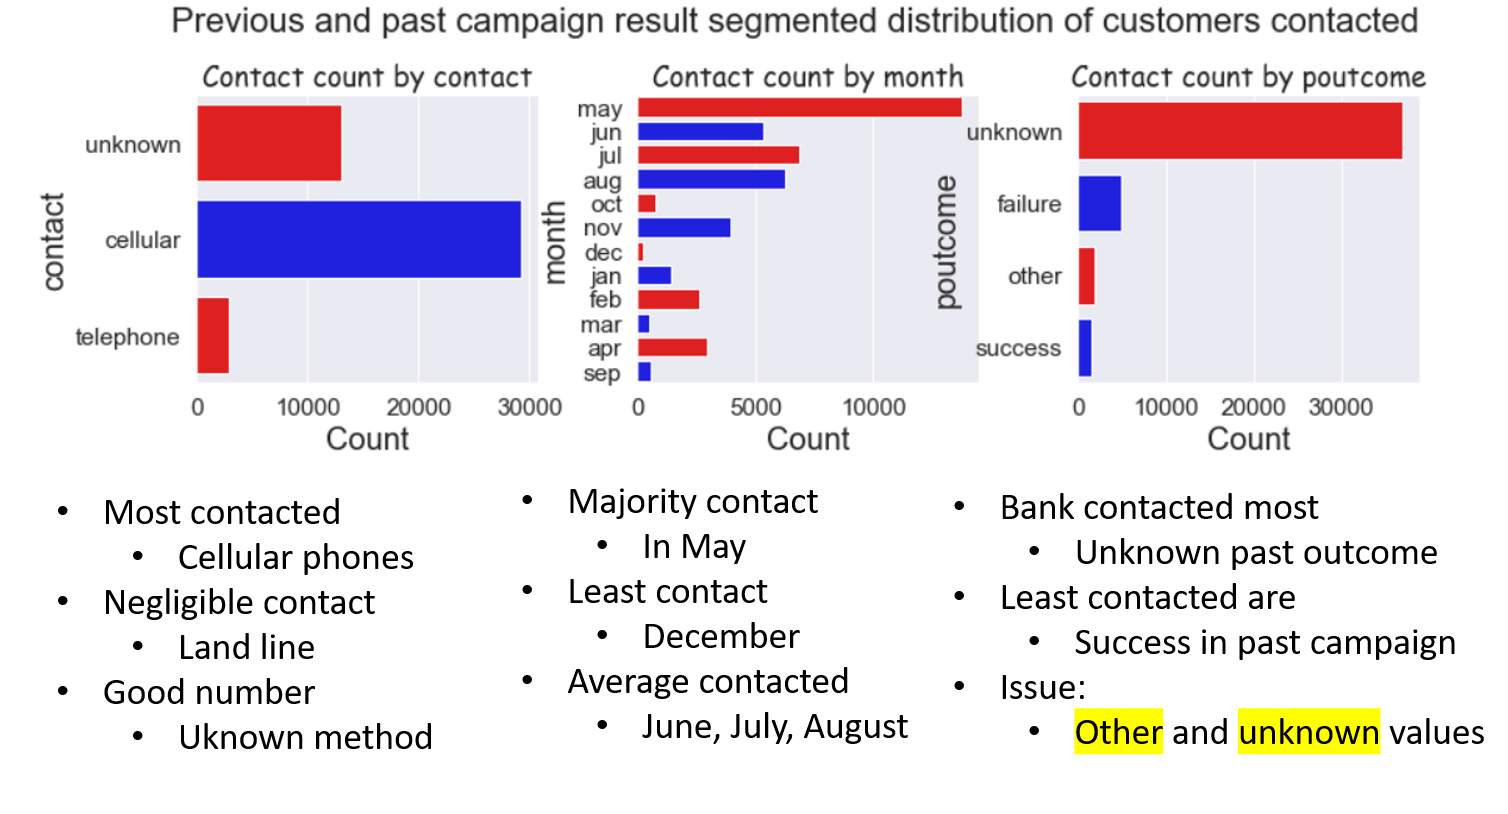
\includegraphics[width=9.50cm]{figures/fig_cat_campaign_count.png}
%		\caption{Single valued features (dropped).}
	\end{figure}
%\end{columns}


\end{frame}


\begin{frame}{Target exploration – class imbalance}
%\linespread{1.3}

%\begin{columns}
%	\column{.6 \textwidth}
%\begin{itemize}
%    \item default - Has credit?
%	\item housing - Has housing loan?
%	\item loan - has personal loan?
%\end{itemize}

%	\column{.4 \textwidth}
	\begin{figure}
		
		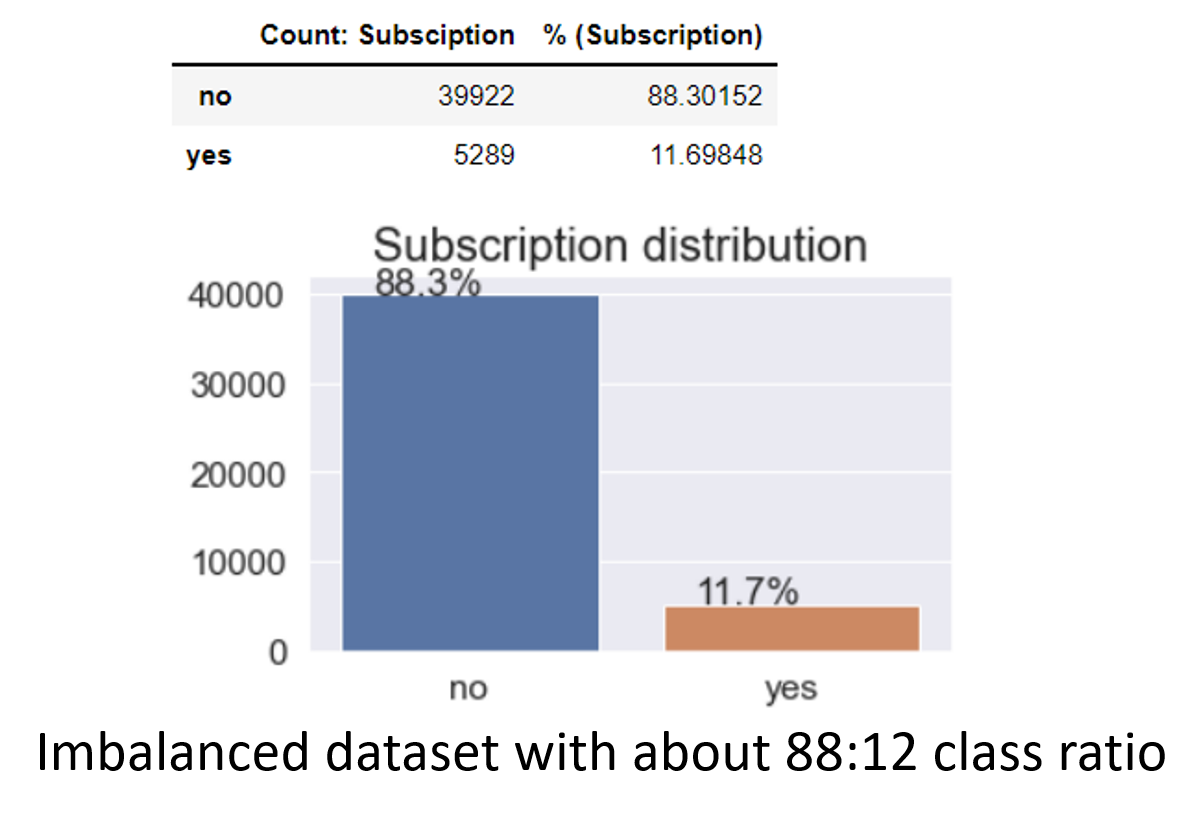
\includegraphics[width=9.50cm]{figures/fig_target_imbalance.png}
%		\caption{Single valued features (dropped).}
	\end{figure}
%\end{columns}


\end{frame}


\begin{frame}{Range of Numerical features – Age and account balance}
%\linespread{1.3}

%\begin{columns}
%	\column{.6 \textwidth}
%\begin{itemize}
%    \item default - Has credit?
%	\item housing - Has housing loan?
%	\item loan - has personal loan?
%\end{itemize}

%	\column{.4 \textwidth}
	\begin{figure}
		
		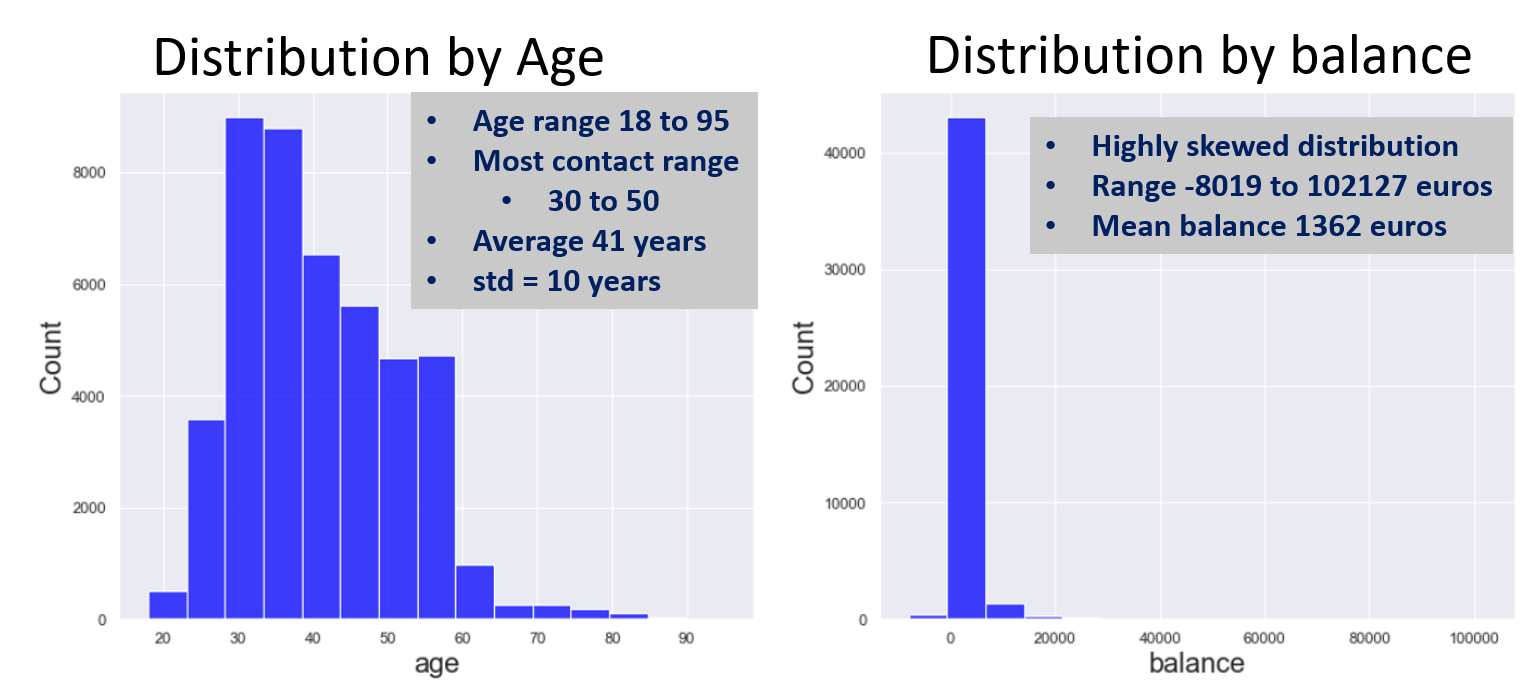
\includegraphics[width=9.50cm]{figures/fig_age_balance_count.png}
%		\caption{Single valued features (dropped).}
	\end{figure}
%\end{columns}


\end{frame}

\begin{frame}{Is balance dependent on age?}
%\linespread{1.3}

%\begin{columns}
%	\column{.6 \textwidth}
%\begin{itemize}
%    \item default - Has credit?
%	\item housing - Has housing loan?
%	\item loan - has personal loan?
%\end{itemize}

%	\column{.4 \textwidth}
	\begin{figure}
		
		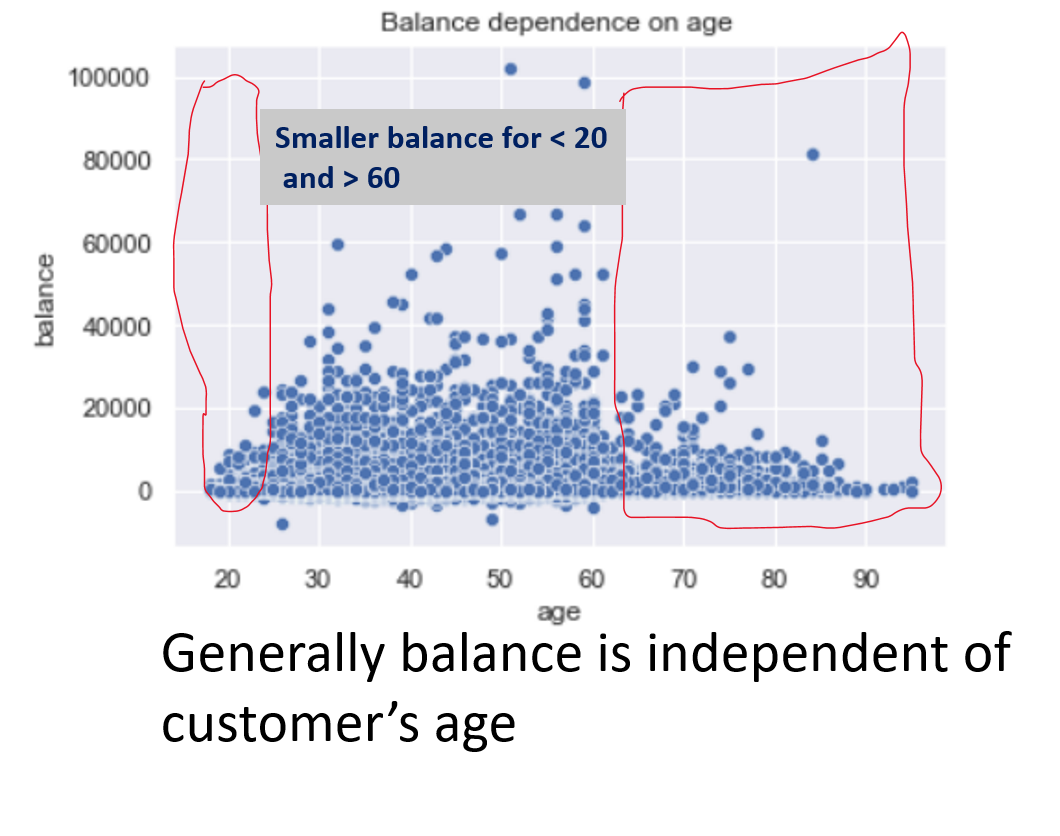
\includegraphics[width=9.50cm]{figures/fig_age_balance_scatter.png}
%		\caption{Single valued features (dropped).}
	\end{figure}
%\end{columns}


\end{frame}


\begin{frame}{Range of Numerical features – Duration and number of contacts}
%\linespread{1.3}

%\begin{columns}
%	\column{.6 \textwidth}
%\begin{itemize}
%    \item default - Has credit?
%	\item housing - Has housing loan?
%	\item loan - has personal loan?
%\end{itemize}

%	\column{.4 \textwidth}
	\begin{figure}
		
		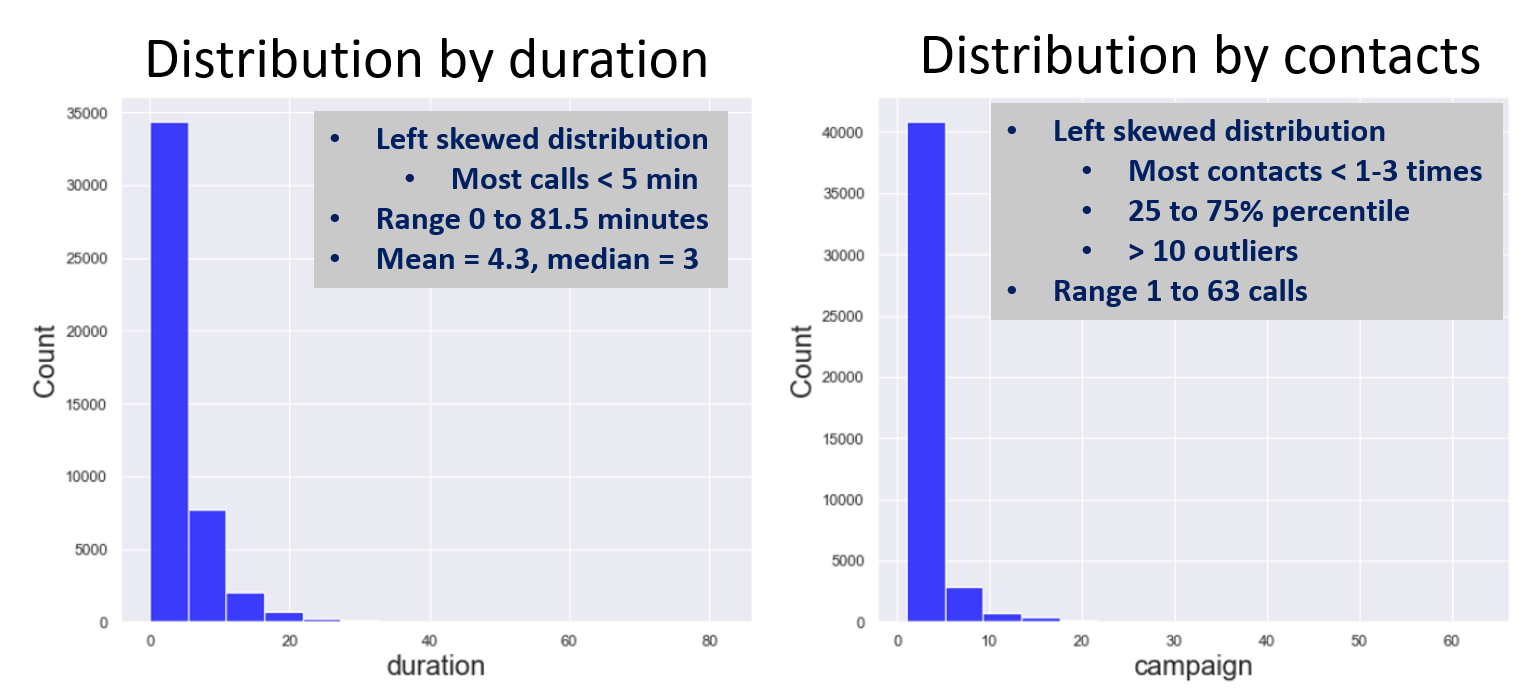
\includegraphics[width=9.50cm]{figures/fig_duration_campaign_count.png}
%		\caption{Single valued features (dropped).}
	\end{figure}
%\end{columns}


\end{frame}


\begin{frame}{Is duration dependent on number of contacts?}
%\linespread{1.3}

%\begin{columns}
%	\column{.6 \textwidth}
%\begin{itemize}
%    \item default - Has credit?
%	\item housing - Has housing loan?
%	\item loan - has personal loan?
%\end{itemize}

%	\column{.4 \textwidth}
	\begin{figure}
		
		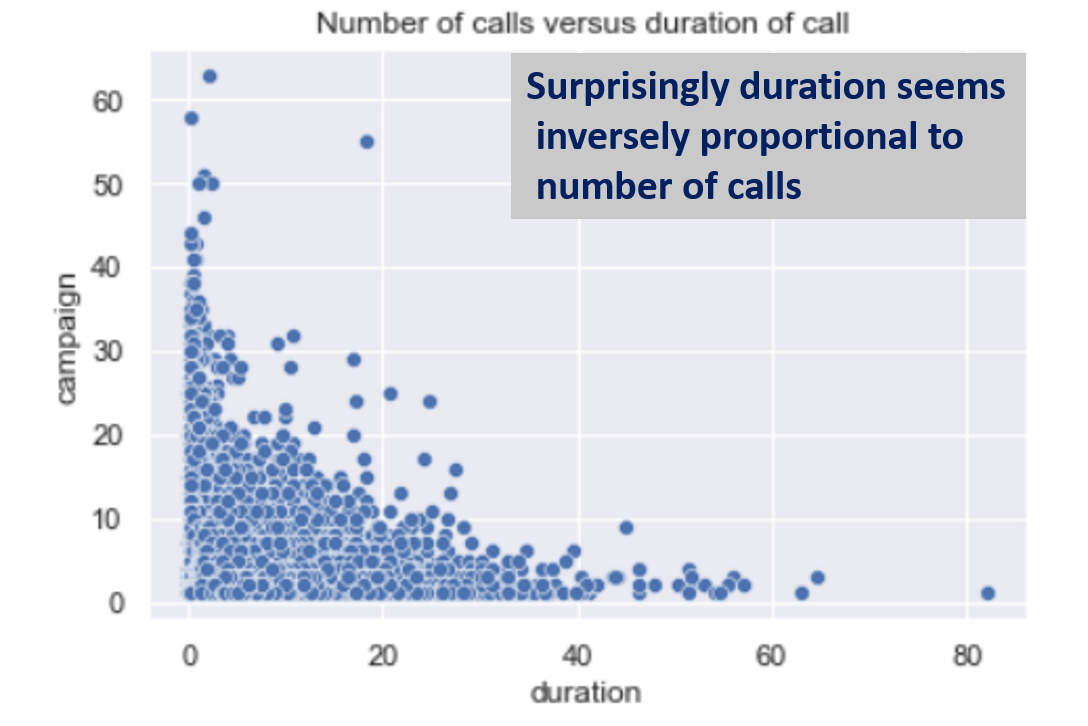
\includegraphics[width=9.50cm]{figures/fig_duration_contact_scatter.png}
%		\caption{Single valued features (dropped).}
	\end{figure}
%\end{columns}


\end{frame}


\begin{frame}{Correlation matrix and interdependence of the numerical features}
%\linespread{1.3}

%\begin{columns}
%	\column{.6 \textwidth}
%\begin{itemize}
%    \item default - Has credit?
%	\item housing - Has housing loan?
%	\item loan - has personal loan?
%\end{itemize}

%	\column{.4 \textwidth}
	\begin{figure}
		
		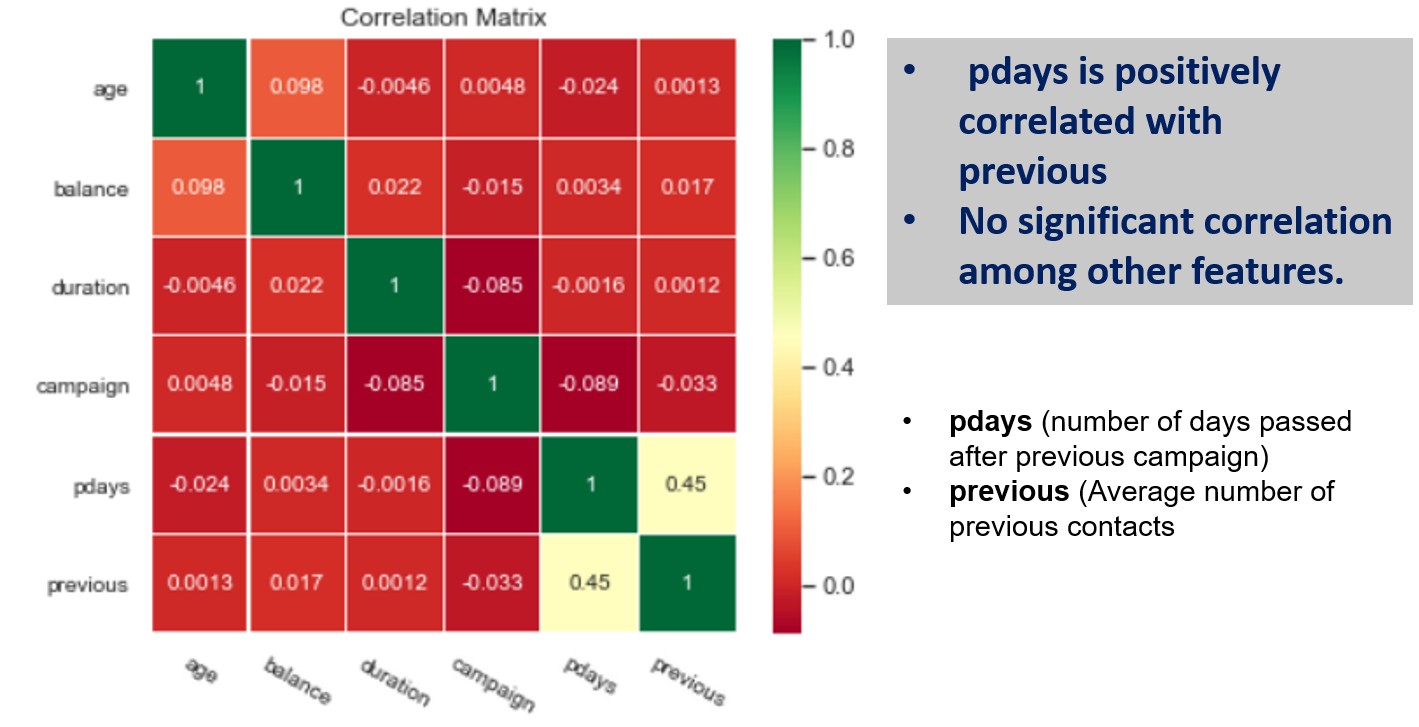
\includegraphics[width=9.50cm]{figures/fig_corr_matrix.png}
%		\caption{Single valued features (dropped).}
	\end{figure}
%\end{columns}

\end{frame}




%%%%%%%%%%%%%%%%%%%%%%%%%%%%%%
%%%%%%%%%%%%%%%%%%%%%%%%%%%%%%
\section{Exploratory Data Analysis} %%%%
%%%%%%%%%%%%%%%%%%%%%%%%%%%%%%
%%%%%%%%%%%%%%%%%%%%%%%%%%%%%%

\begin{frame}{Objectives of Exploratory Data Analysis}
%\linespread{1.3}
\begin{itemize}
    \item Examine effect of each feature on target (subscription rate)
    \item Identify feature groups that maximize subscription rate
    \item Make recommendation for our client
\end{itemize}
%\begin{figure}
		%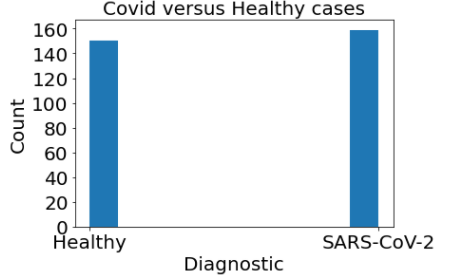
\includegraphics[width=7.0cm]{balance.png}
		%\caption{$\approx 50:50$ COVID to Healthy class ratio.}
	%\end{figure}

\end{frame}


\begin{frame}{Effect of customer job on subscription rate}
%\linespread{1.3}

%\begin{columns}
%	\column{.6 \textwidth}
%\begin{itemize}
%    \item default - Has credit?
%	\item housing - Has housing loan?
%	\item loan - has personal loan?
%\end{itemize}

%	\column{.4 \textwidth}
	\begin{figure}
		
		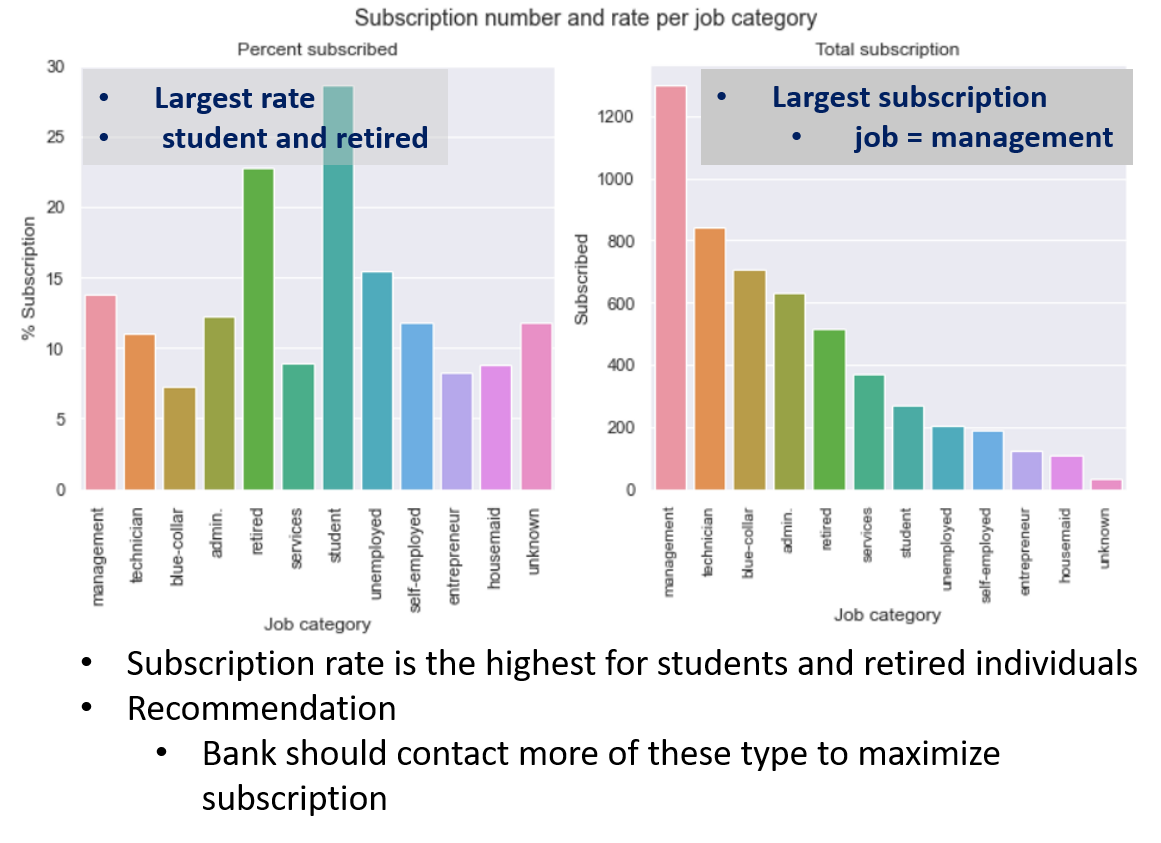
\includegraphics[width=9.50cm]{figures/fig_job_rate.png}
%		\caption{Single valued features (dropped).}
	\end{figure}
%\end{columns}


\end{frame}


\begin{frame}{Effect of marital status and educational level on subscription rate}
%\linespread{1.3}

%\begin{columns}
%	\column{.6 \textwidth}
%\begin{itemize}
%    \item default - Has credit?
%	\item housing - Has housing loan?
%	\item loan - has personal loan?
%\end{itemize}

%	\column{.4 \textwidth}
	\begin{figure}
		
		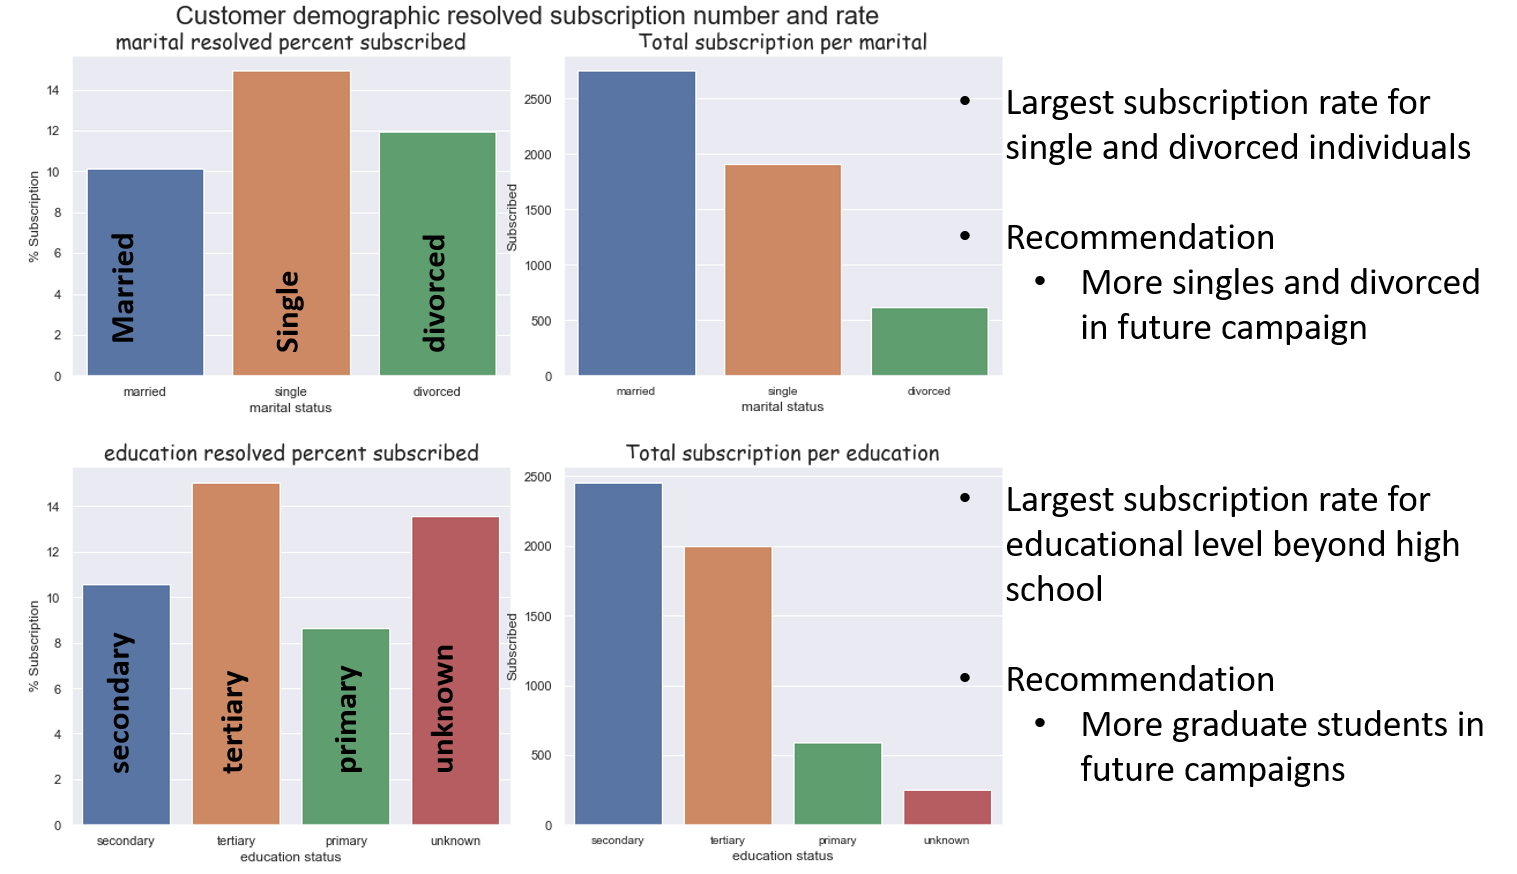
\includegraphics[width=9.50cm]{figures/fig_marital_education_rate.png}
%		\caption{Single valued features (dropped).}
	\end{figure}
%\end{columns}


\end{frame}


\begin{frame}{Effect of financial profile on subscription rate}
%\linespread{1.3}

%\begin{columns}
%	\column{.6 \textwidth}
%\begin{itemize}
%    \item default - Has credit?
%	\item housing - Has housing loan?
%	\item loan - has personal loan?
%\end{itemize}

%	\column{.4 \textwidth}
	\begin{figure}
		
		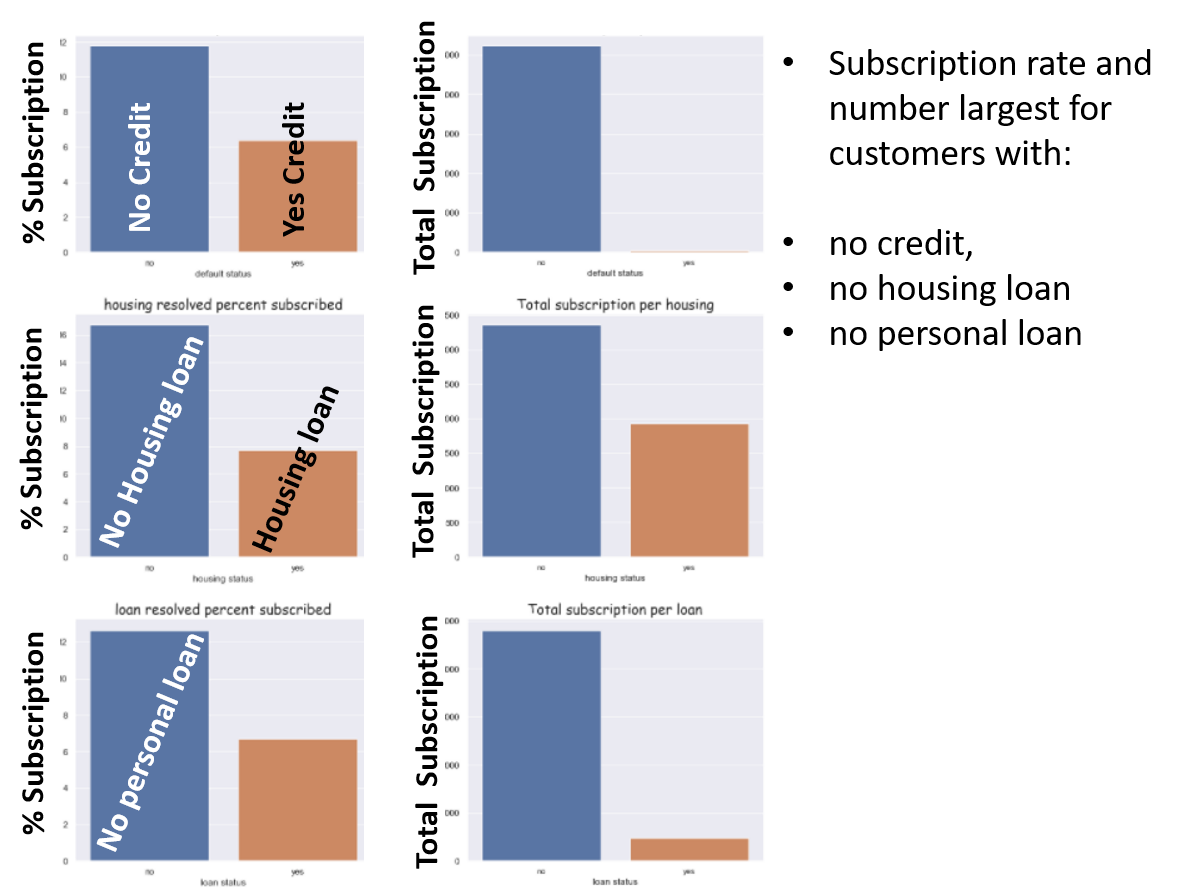
\includegraphics[width=9.50cm]{figures/fig_financial_rate.png}
%		\caption{Single valued features (dropped).}
	\end{figure}
%\end{columns}
\end{frame}

\begin{frame}{Effect of age and account balance on subscription rate}
%\linespread{1.3}

%\begin{columns}
%	\column{.6 \textwidth}
%\begin{itemize}
%    \item default - Has credit?
%	\item housing - Has housing loan?
%	\item loan - has personal loan?
%\end{itemize}

%	\column{.4 \textwidth}
	\begin{figure}
		
		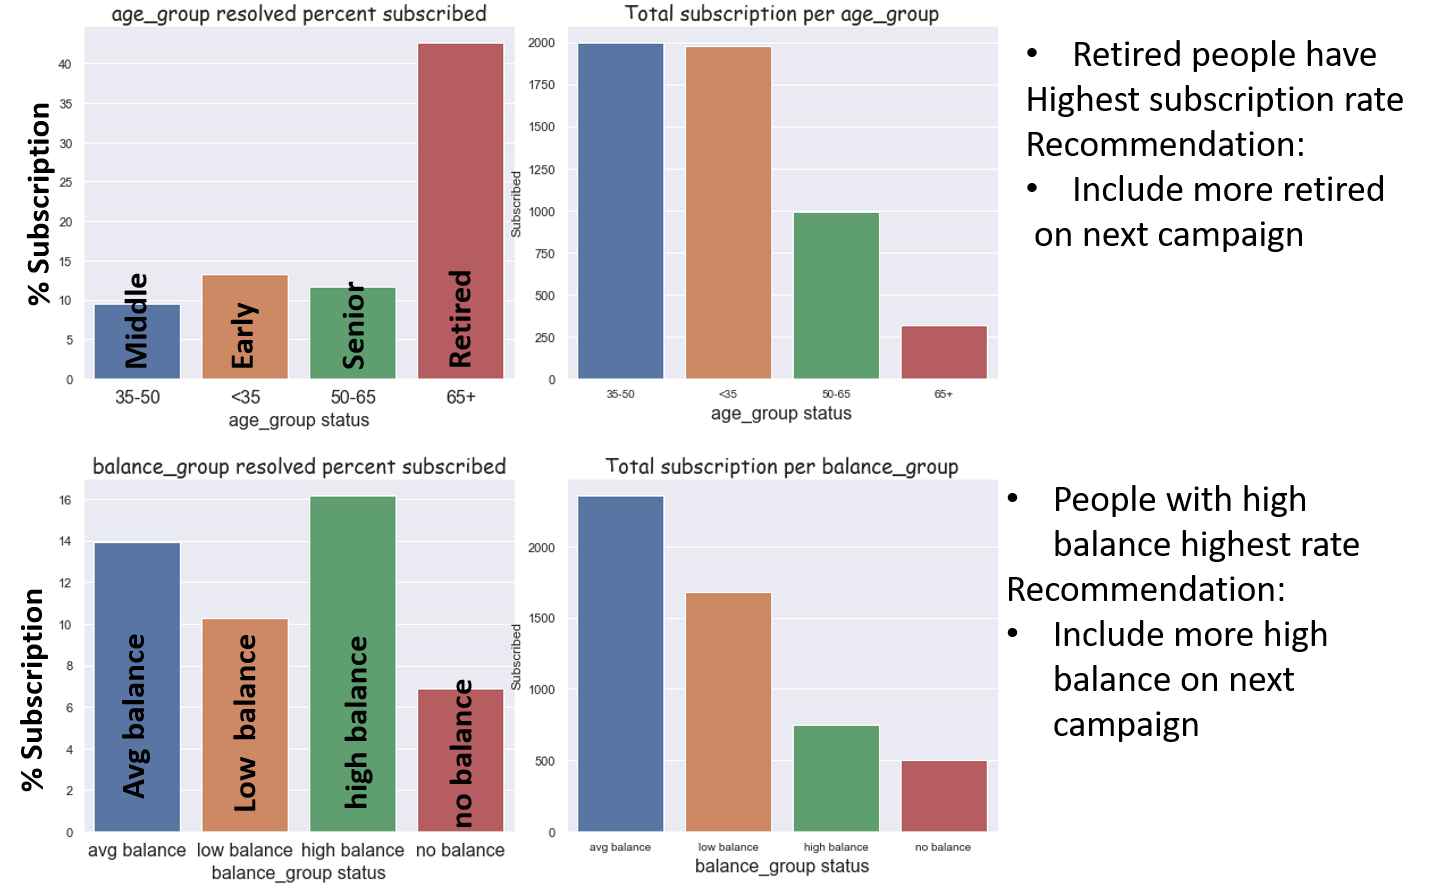
\includegraphics[width=9.50cm]{figures/fig_age_balance_rate.png}
%		\caption{Single valued features (dropped).}
	\end{figure}
%\end{columns}
\end{frame}

%%%%%%%%%%%%%%%%%%%%%%%Preprocessing%%%%%%%%%%%%%%%%%%%%%%%%%%%%%%
\section{Preprocessing} %%%%
%%%%%%%%%%%%%%%%%%%%%%%%%%%%%%
%%%%%%%%%%%%%%%%%%%%%%%%%%%%%%

\begin{frame}{Schematics of data pre-processing}
%\linespread{1.3}
Data pre-processing included:
\begin{itemize}
    \item Load clean dataset
    \item Transform categorical features 
    \item Handle class imbalance
\end{itemize}
\begin{figure}
		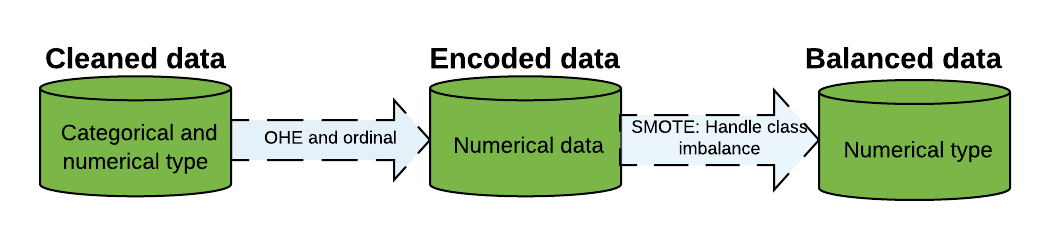
\includegraphics[width=9.0cm]{figures/preprocessing.png}
		%\caption{$\approx 50:50$ COVID to Healthy class ratio.}
	\end{figure}
%\center{All models seem to over-fit.}
%\center{\textcolor{blue}{Need to be tested with the test split.}}
\end{frame}

\begin{frame}{Transform categorical features to numerical types}
%\linespread{1.3}
Features transformed with:
\begin{itemize}
    \item Ordinal encoding (number of labels = 2)
    \item One hot encoding (number of labels > 2) 
\end{itemize}
\begin{figure}
		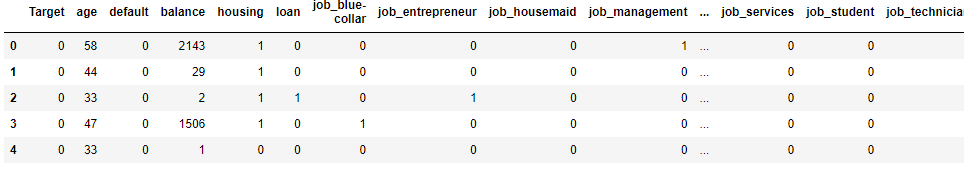
\includegraphics[width=9.0cm]{figures/fig_df_OHE.PNG}
		\caption{Preview of data transformed into numerical values}
	\end{figure}
%\center{All models seem to over-fit.}
%\center{\textcolor{blue}{Need to be tested with the test split.}}
\end{frame}

\begin{frame}{Data imbalance handled with SMOTE: Synthetic Minority Oversampling Technique}
%\linespread{1.3}
Data balanced with SMOTE shows 50:50 class ratio::
\begin{figure}
		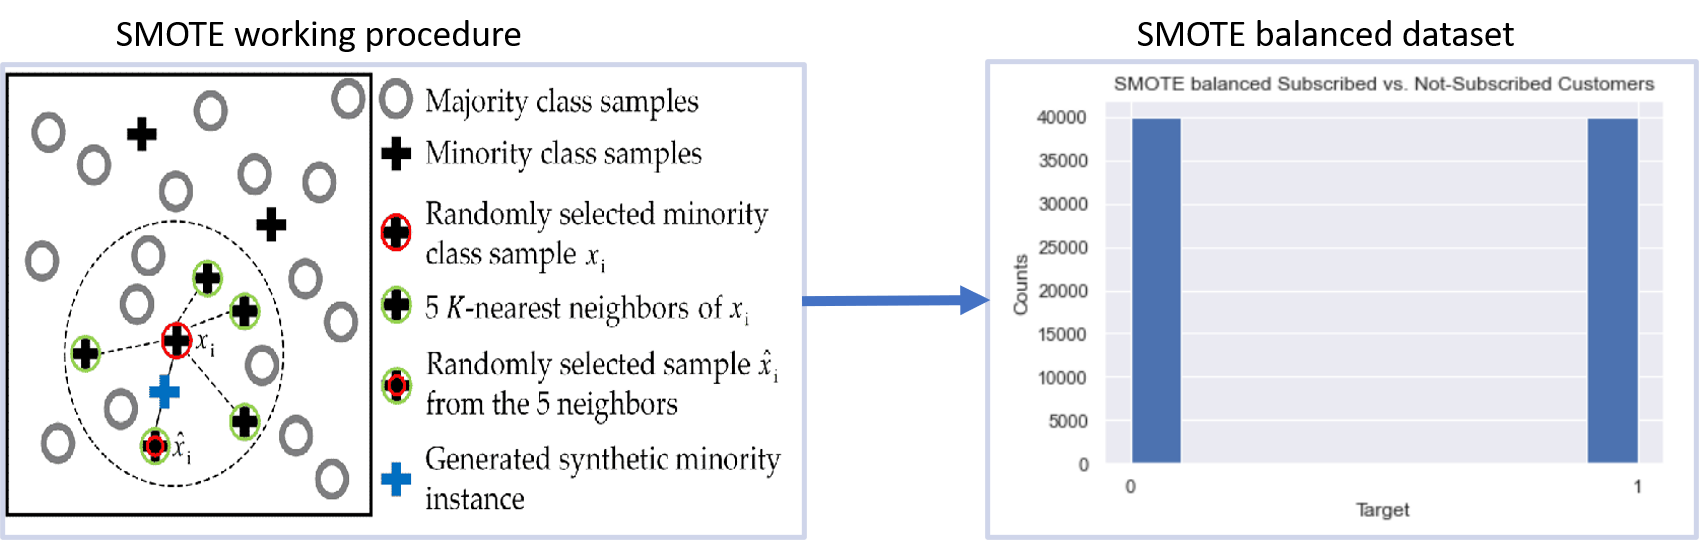
\includegraphics[width=9.0cm]{figures/fig_smote_and_data.png}
%		\caption{Preview of data transformed into numerical values}
	\end{figure}
%\center{All models seem to over-fit.}
%\center{\textcolor{blue}{Need to be tested with the test split.}}
\end{frame}





%%%%%%%%%%%%%%%%%%%%%%%%%%%%%%
%%%%%%%%%%%%%%%%%%%%%%%%%%%%%%
\section{Modeling} %%%%
%%%%%%%%%%%%%%%%%%%%%%%%%%%%%%
%%%%%%%%%%%%%%%%%%%%%%%%%%%%%%

\begin{frame}{Schematics of machine learning modeling}
%\linespread{1.3}
%Three models considered:
%\begin{itemize}
%    \item Decision tree
%    \item Logistic regression
%    \item Random forest
%\end{itemize}
\begin{figure}
		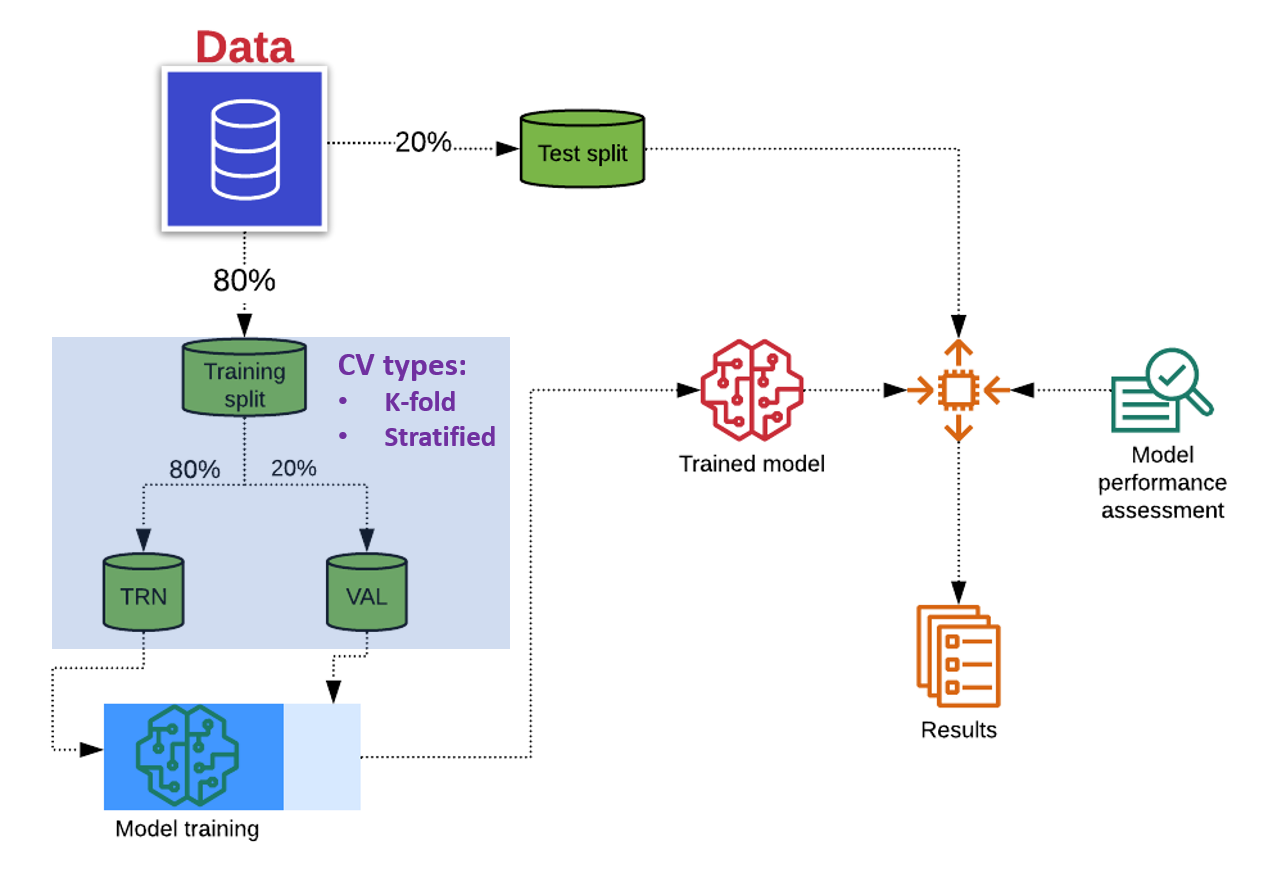
\includegraphics[width=9.8cm]{figures/fig_model_schematics.png}
		%\caption{$\approx 50:50$ COVID to Healthy class ratio.}
	\end{figure}
%\center{All models seem to over-fit.}
%\center{\textcolor{blue}{Need to be tested with the test split.}}
\end{frame}

\begin{frame}{Machine learning model type corresponding to our domain problem}
%\linespread{1.3}
%Three models considered:
%\begin{itemize}
%    \item Decision tree
%    \item Logistic regression
%    \item Random forest
%\end{itemize}
\begin{figure}
		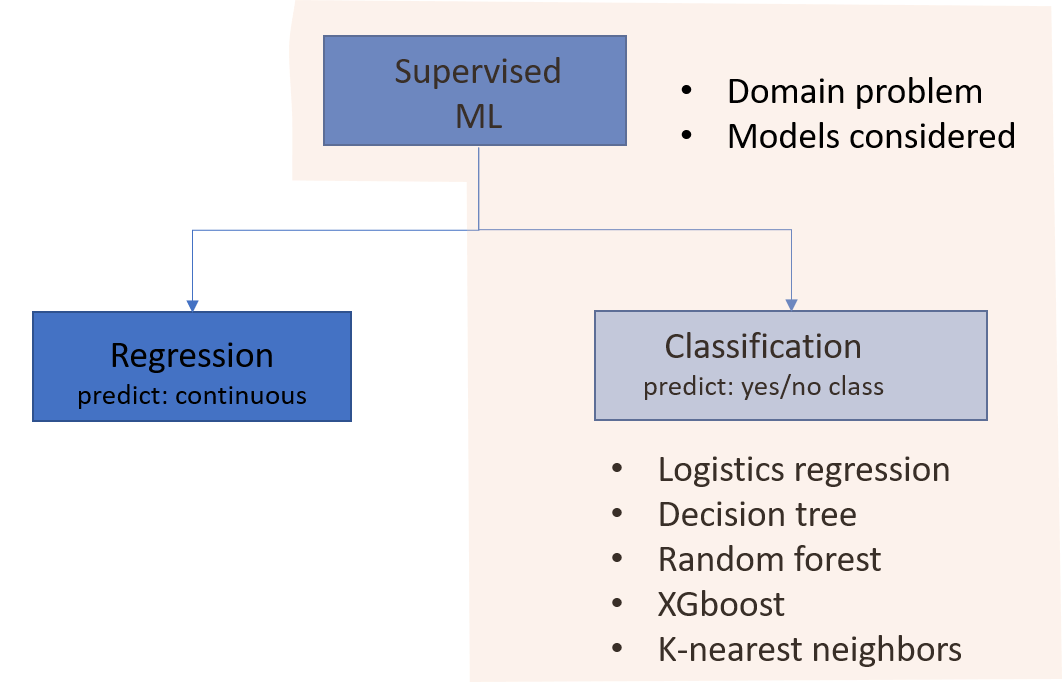
\includegraphics[width=9.5cm]{figures/fig_model_domain.png}
		%\caption{$\approx 50:50$ COVID to Healthy class ratio.}
	\end{figure}
%\center{All models seem to over-fit.}
%\center{\textcolor{blue}{Need to be tested with the test split.}}
\end{frame}

\begin{frame}{Stratified K-fold Cross validation results to marginal improvement of model performance}
%\linespread{1.3}

%\begin{itemize}
%  \item 70\% AUC score and 88\% Accuracy
%    \item Logistic regression
%    \item Random forest
%\end{itemize}
\begin{figure}
		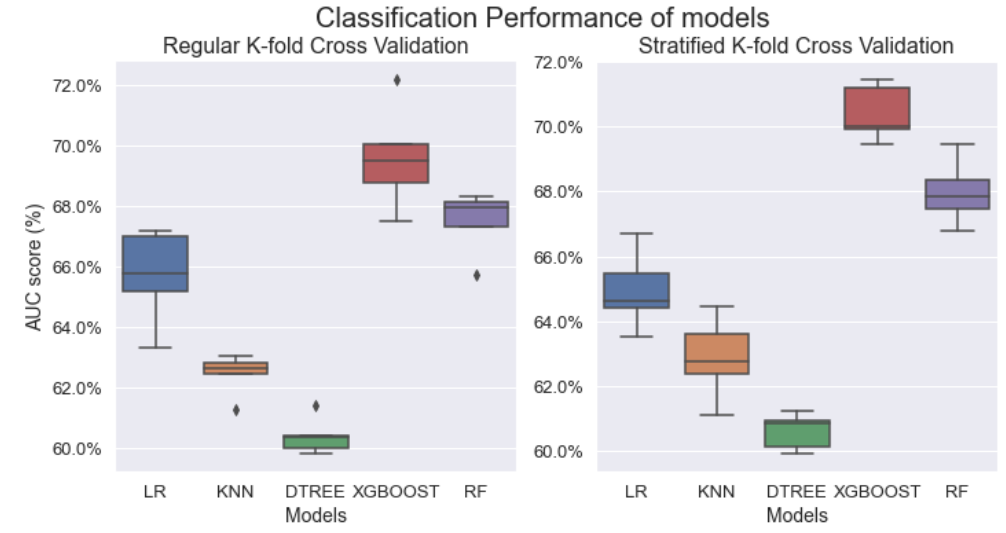
\includegraphics[width=9.50cm]{figures/fig_regular_vs_stratified_kfold.PNG}
		%\caption{$\approx 50:50$ COVID to Healthy class ratio.}
	\end{figure}
%\center{All models seem to over-fit.}
%\center{\textcolor{blue}{Need to be tested with the test split.}}
\end{frame}

\begin{frame}{Data imbalance handled with SMOTE resulted to significant performance increase}
%\linespread{1.3}

%\begin{itemize}
%  \item 70\% AUC score and 88\% Accuracy
%    \item Logistic regression
%    \item Random forest
%\end{itemize}
\begin{figure}
		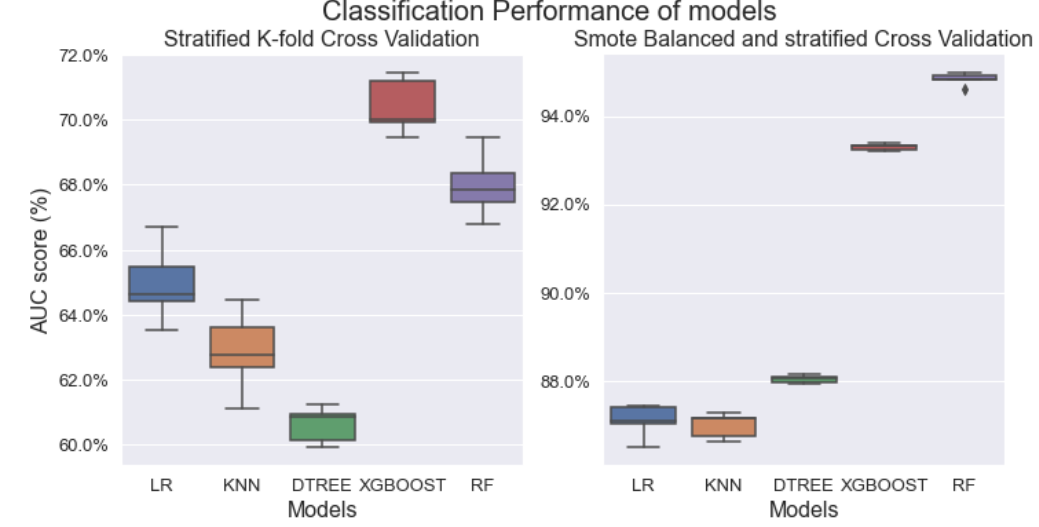
\includegraphics[width=9.80cm]{figures/fig_kfold_vs_smote.PNG}
		%\caption{$\approx 50:50$ COVID to Healthy class ratio.}
	\end{figure}
%\center{All models seem to over-fit.}
%\center{\textcolor{blue}{Need to be tested with the test split.}}
\end{frame}

\begin{frame}{Hyperparameter tuning resulted in a stable model with slight performance improvement}
%\linespread{1.3}

%\begin{itemize}
%  \item 70\% AUC score and 88\% Accuracy
%    \item Logistic regression
%    \item Random forest
%\end{itemize}
%\begin{figure}
\begin{picture}(100,100)
\put(0,-80){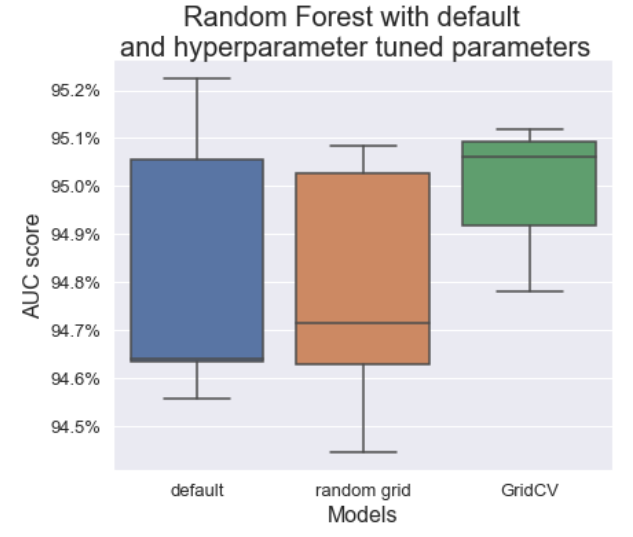
\includegraphics[width=9.0cm]{figures/fig_default_vs_tuned.PNG}}
		%\caption{$\approx 50:50$ COVID to Healthy class ratio.}
%\end{figure}
\put(70,10){\textcolor{red}{\textbf{}}}
\end{picture}
%\center{All models seem to over-fit.}
%\center{\textcolor{blue}{Need to be tested with the test split.}}
\end{frame}


%\begin{frame}{Cross-validation model performance with ROC-AUC metric}
%\linespread{1.3}
%XGBOOST is Best performing model:
%\begin{itemize}
%  \item 70\% AUC score and 88\% Accuracy
%    \item Logistic regression
%    \item Random forest
%\end{itemize}
%\begin{figure}
		%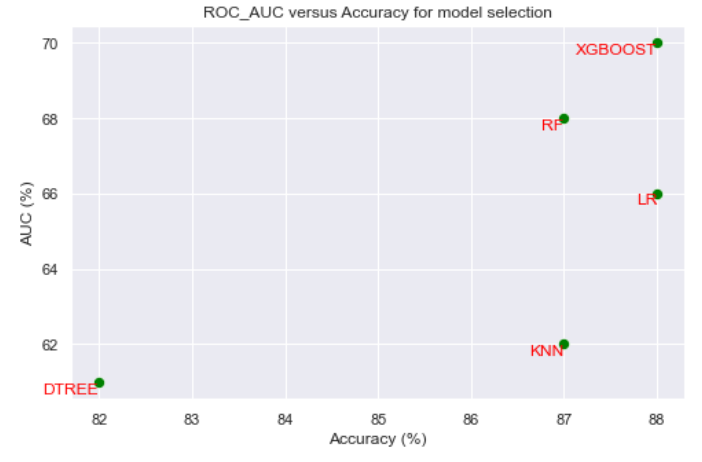
\includegraphics[width=9.0cm]{figures/fig_auc_vs_accuracy.PNG}
		%\caption{$\approx 50:50$ COVID to Healthy class ratio.}
	%\end{figure}
%\center{All models seem to over-fit.}
%\center{\textcolor{blue}{Need to be tested with the test split.}}
%\end{frame}

\begin{frame}{Best Random Forest performance on the test set}
%\linespread{1.3}
Grid optimized Random Forest performance on the test set:
\begin{itemize}
  \item AUC score: 95.1\%
%    \item Logistic regression
%    \item Random forest
\end{itemize}
\begin{figure}
		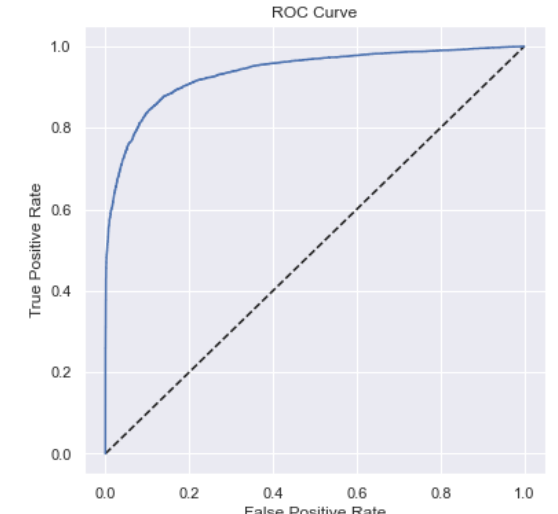
\includegraphics[width=7.0cm]{figures/fig_xgboos_roc.PNG}
		%\caption{$\approx 50:50$ COVID to Healthy class ratio.}
	\end{figure}
%\center{All models seem to over-fit.}
%\center{\textcolor{blue}{Need to be tested with the test split.}}
\end{frame}

\begin{frame}{Feature importance of Best random forest model}
%\linespread
Most important 3 features for term deposit subscription are:
\begin{itemize}
  \item \textbf{balance}: Amount of customer account balance
    \item \textbf{age}: Age of customer
    \item \textbf{housing loan:} Has housing loan?
\end{itemize}
\begin{figure}
		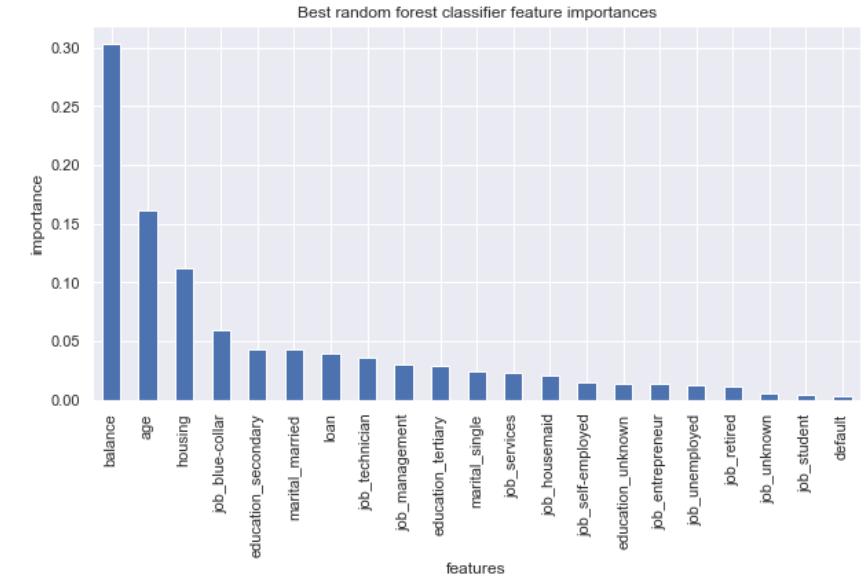
\includegraphics[width=8.0cm]{figures/fig_feature_importance_rf.PNG}
		%\caption{$\approx 50:50$ COVID to Healthy class ratio.}
	\end{figure}
%\center{All models seem to over-fit.}
%\center{\textcolor{blue}{Need to be tested with the test split.}}
\end{frame}




%%%%%%%%%%%%%%%%%%%%%%%%%%%%%%
%%%%%%%%%%%%%%%%%%%%%%%%%%%%%%
\section{Summary} %%%%
%%%%%%%%%%%%%%%%%%%%%%%%%%%%%%
%%%%%%%%%%%%%%%%%%%%%%%%%%%%%%


\begin{frame}{Summary and Future Work}
\linespread{1.3}

\begin{itemize}
    \item We developed supervised machine learning models for predicting customer subscription to term deposit.
    \item Logistic regression, decision tree, random forest, XGboos, and K-nearest neighbours machine learning algorithms considered. 
    \item We find customer subscription to term deposit can be predicted using Random Forest with an AUC score of 95\%.
    \item Future regression machine learning work needs to be completed to predict time spent talking to targeted customers.
    
\end{itemize}


\end{frame}


%%%%%%%%%%%%%%%%%%%%%%%%%%%%%%
%%%%%%%%%%%%%%%%%%%%%%%%%%%%%
\section{Acknowledgement} %%%%
%%%%%%%%%%%%%%%%%%%%%%%%%%%%%%
%%%%%%%%%%%%%%%%%%%%%%%%%%%%%%

\begin{frame}{Acknowledgement}
\linespread{1.3}

\center{\textbf{Springboard mentor:} Yuxuan Xin}
\center{for time generous and insightful discussions}

\end{frame}






\end{document}
